% Authoritative TikZ source for the website project-workflow figure.
\documentclass[tikz,border=6pt]{standalone}
\usetikzlibrary{arrows.meta,positioning}
\definecolor{HLTeal}{HTML}{157C87}
\definecolor{HLPink}{HTML}{BD1763}
\definecolor{HLGold}{HTML}{D6A700}
\definecolor{HLSoft}{HTML}{F8F5F7}
\begin{document}
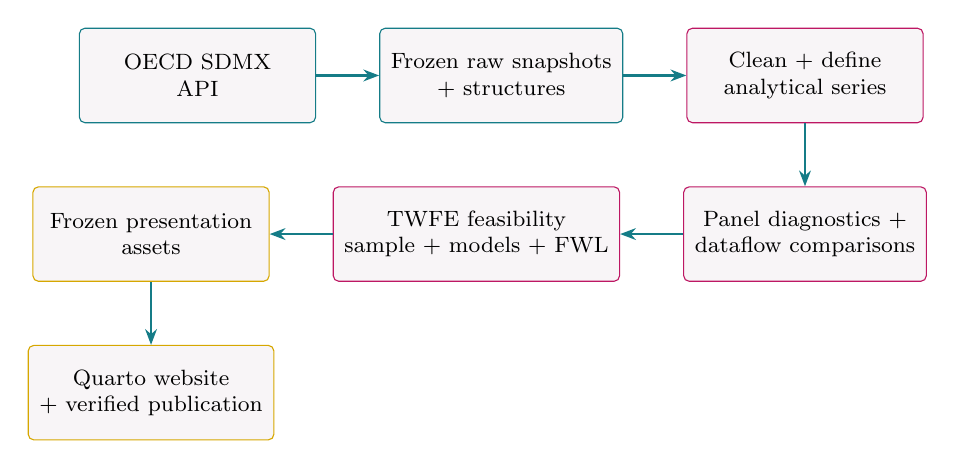
\begin{tikzpicture}[font=\sffamily, node distance=8mm and 8mm,
  stage/.style={draw=HLTeal, rounded corners=2pt, fill=HLSoft, minimum width=30mm, minimum height=12mm, align=center, inner sep=4pt, font=\footnotesize},
  analysis/.style={stage, draw=HLPink}, publish/.style={stage, draw=HLGold},
  flow/.style={-{Stealth[length=2mm]}, thick, draw=HLTeal}]
\node[stage] (api) {OECD SDMX\\API};
\node[stage, right=of api] (snap) {Frozen raw snapshots\\+ structures};
\node[analysis, right=of snap] (prep) {Clean + define\\analytical series};
\node[analysis, below=of prep] (diag) {Panel diagnostics +\\dataflow comparisons};
\node[analysis, left=of diag] (twfe) {TWFE feasibility\\sample + models + FWL};
\node[publish, left=of twfe] (pres) {Frozen presentation\\assets};
\node[publish, below=of pres] (site) {Quarto website\\+ verified publication};
\draw[flow] (api) -- (snap); \draw[flow] (snap) -- (prep); \draw[flow] (prep) -- (diag);
\draw[flow] (diag) -- (twfe); \draw[flow] (twfe) -- (pres); \draw[flow] (pres) -- (site);
\end{tikzpicture}
\end{document}
